\subsection{Peking}

Al realizar el experimento, se logró llegar al destino en el ttl 29. De estos, 4 no respondieron. Los ttls que Cimbala reconoció como intercontinentales fueron 6, 10, 12, 14, 15, 20, 21.

\begin{figure}[h!]
  \centering
    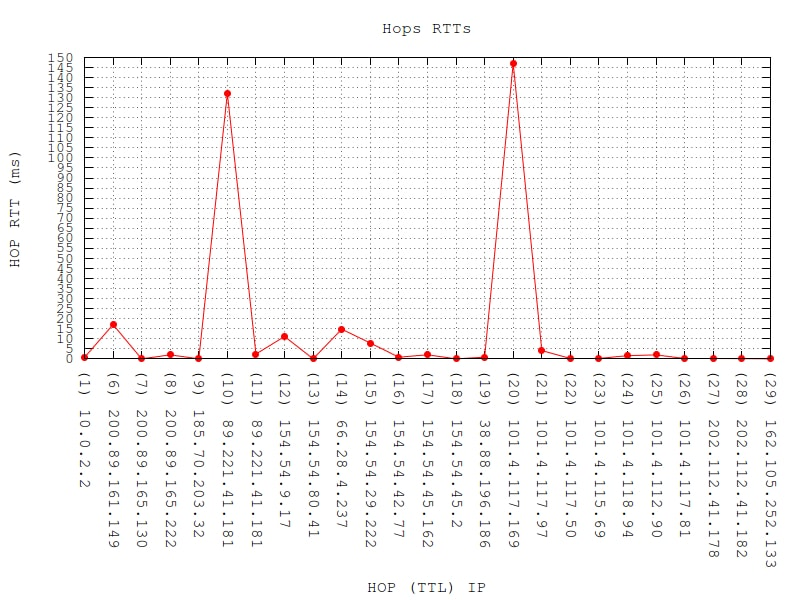
\includegraphics[scale=0.6]{imagenes/peking-graficos/traceroute-peking.jpg}
  \caption{peking- RTT hops}
  \label{fig:10}
\end{figure}

En la figura \ref{fig:10} se puede observar como el ttl 10 y 20 tienen un rtt claramente distinguido del resto.

\begin{figure}[h!]
  \centering
    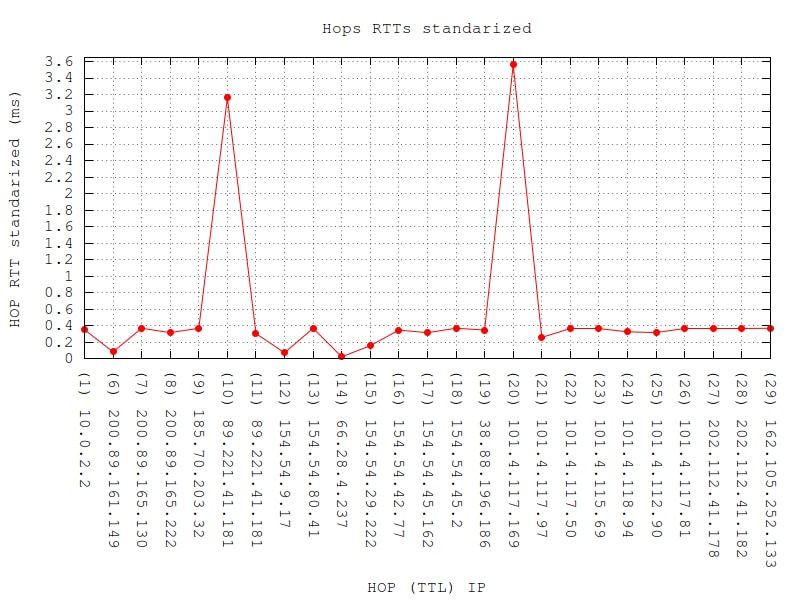
\includegraphics[scale=0.6]{imagenes/peking-graficos/traceroute-peking-standarized.jpg}
  \caption{peking- RTT hops standarized}
  \label{fig:11}
\end{figure}

En la figura \ref{fig:11} se puede observar una situacion similar a la de la figura \ref{fig:10}.

